
\section{HiFloat4}

This section provides a systematic description of the proposed 4-bit BFP 
format HiF4, and details its structural components. 
We then present the conversion algorithm from BF16 to HiF4, 
along with the suggested hardware support. 

\subsection{Format Definition}
As shown in Figure \ref{HiF4-Structure}, a basic HiF4 unit consists of 
32 bits shared scaling metadata, and 64 4-bit in-group elements, 
resulting in an average storage of 4.5 bits per value. 
The following defines each component in detail. 

\begin{figure}[htbp]
  \centering
  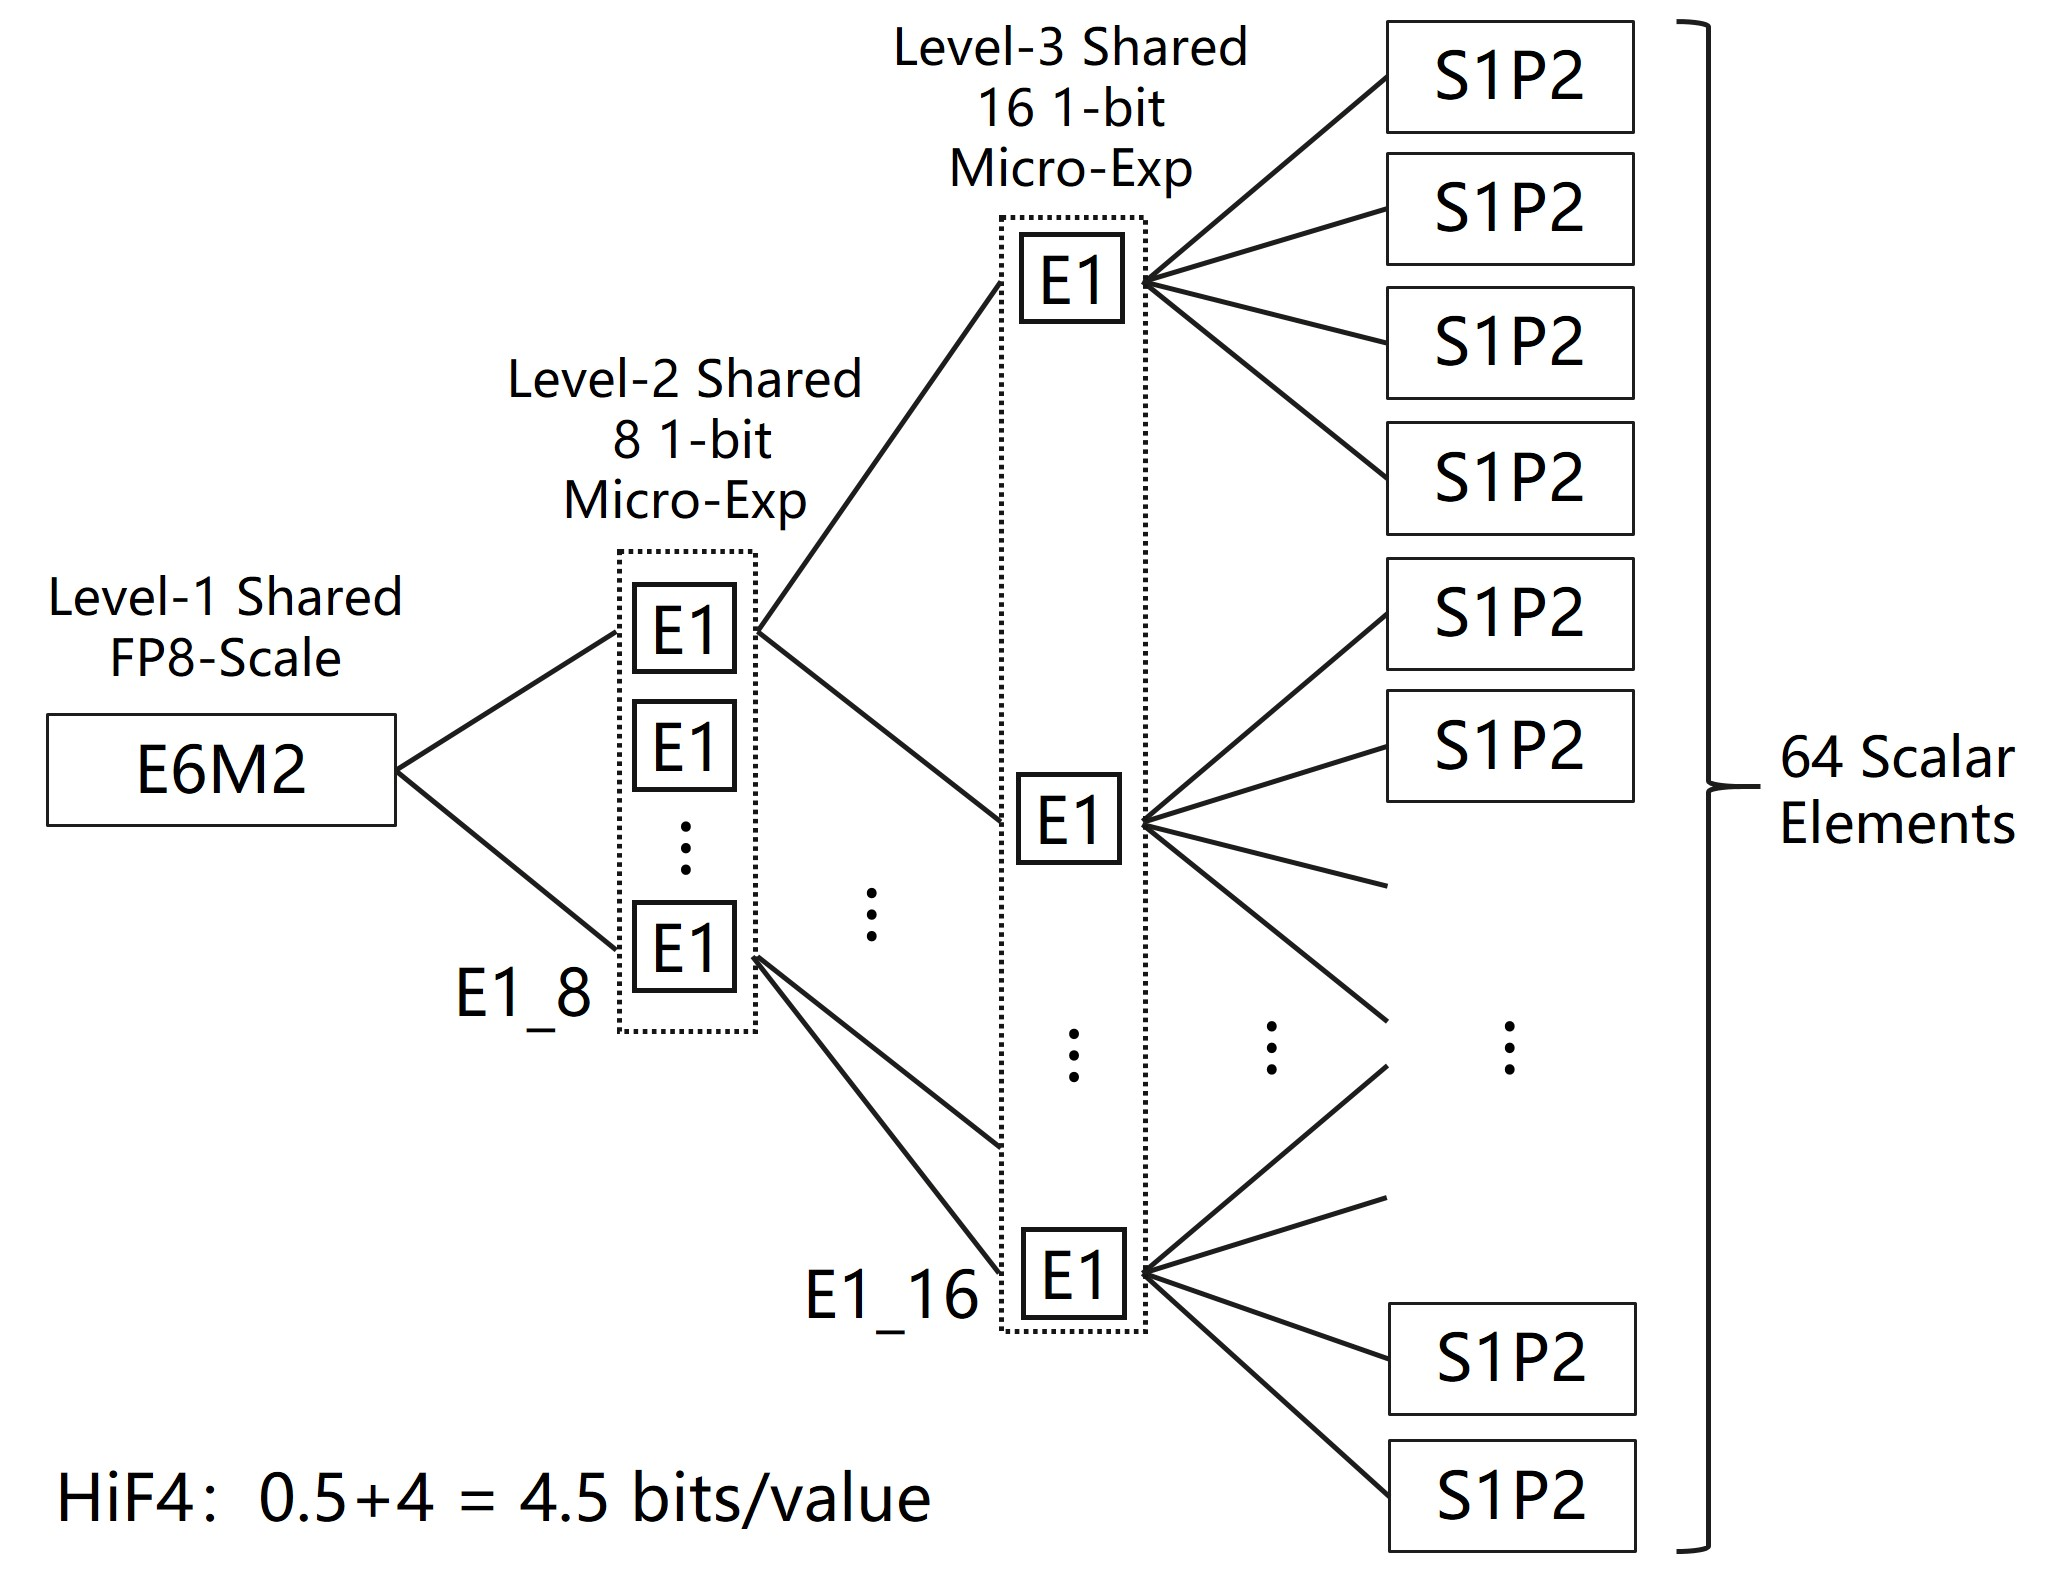
\includegraphics[width=\linewidth]{Fig/HiF4-Structure.jpg}
  \caption{The Structure of HiF4 Block Floating-Point Format}
  \label{HiF4-Structure}
\end{figure}

\subsubsection{Scaling Metadata}

The metadata defines a three-level scaling hierarchy. 
The first level (E6M2) is a specially designed unsigned 8-bit 
floating-point format. 
This scale provides a wide dynamic range across groups and normalizes 
each group's peak magnitude to the representable upper bound of the 
remaining hierarchical format structure, 
ensuring full utilization of the intra-group dynamic range. 
Table \ref{E6M2-S1P2} summarizes the encoding details of E6M2. 
We assign 6 bits to the exponent field with a bias of 48, and 2 bits 
to the mantissa field with one hidden integer bit set to 1. 
E6M2 encodes NaN (Not a Number) but no other special values such 
as infinity or zero. 
Meanwhile, only normal mode is supported. 
Thus if we denote the unbiased exponent as E and the mantissa 
as M, an E6M2 number used in HiF4 should be interpreted as follows: 
\begin{equation}
  X = 2^{E} \times 1.M       \label{E6M2-Eq}
\end{equation} 
The second (E1\_8) and third (E1\_16) levels, implemented as 8-way 
and 16-way 1-bit micro-exponents, expand the intra-group dynamic 
range by refining local exponent differences, 
effectively mitigating the impact of outliers and suppressing 
quantization error. 
Micro-exponent E1 directly encodes 1 and 0, representing a very  
fine-grained power-of-two scaling factor. 
In this hierarchical scaling scheme, 
the level-1 E6M2 factor provides a global base scale connected to 
all level-2 micro-exponents. 
Each level-2 E1 further connects to two adjacent third-level 
micro-exponents, 
while each level-3 E1 in turn connects to four contiguous 4-bit 
elements within its local group. 
All three-level scaling metadata occupies 32 bits, 
distributed over 64 in-group elements, 
leading to an extra overhead of 0.5 bits per value. 

\begin{table}[tbp]
  \caption{E6M2 and S1P2 Encoding Details}
  \label{E6M2-S1P2}
  \centering
  \begin{tabular}{lll}
    \toprule 
     & Unsigned FP8-E6M2 & Sign-Magnitude S1P2\\
    \midrule
    Exponent Bias     & 48                                   & N/A    \\
    Unbiased Exp      & [-48, 15]                            & N/A    \\
    Infinity          & N/A                                  & N/A    \\
    Zero              & N/A                                  & S$0.00_2 = \pm 0.00$ \\
    NaN               & $111111\_ 11_2$                      & N/A    \\
    Max Value         & $111111\_10_2 = 2^{15} \times 1.50$  & S$1.11_2 = \pm 1.75$ \\
    Min Value         & $000000\_00_2 = 2^{-48} \times 1.00$ & S$0.01_2 = \pm 0.25$ \\
    \bottomrule
  \end{tabular}
\end{table}

\subsubsection{Element Encoding}

HiF4 encodes the 4-bit in-group elements using the 
sign-magnitude S1P2 representation. 
In this SXPY notation, S denotes the sign bit and P indicates the 
binary point. 
The value X preceding P designates a X-bit integer part, whereas 
the value Y following P designates a Y-bit fractional part. 
The encoding details of S1P2 are summarized in Table \ref{E6M2-S1P2}. 
Conceptually, S1P2 is equivalent to the E1M2 format in floating-point 
representation; 
however, we adopt the S1P2 notation because it is more intuitive to 
interpret.

\subsubsection{Represented Values}

Since we have elaborated on each component, 
we can now look at the HiF4 unit as a whole and 
compute its represented values. 
As depicted in Figure \ref{HiF4-Structure}, 
a single group in the HiF4 format comprises four 
levels of data, 
which are related through multiplication. 
Let $\{S1P2\}_i$ denote the i-th in-group element 
value, where i $\in$ [1, 64].
Let $\{E1\_8\}_j$ denote the j-th micro-exponent in the 
level-2 scaling metadata, where j $\in$ [1, 8]. 
Similarly, let $\{E1\_16\}_k$ denote the k-th 
micro-exponent in the level-3 scaling metadata, 
where k $\in$ [1, 16]. 
Finally, let $\{V_i\}_{i=1}^{64}$ represent the 64 real 
numbers in a HiF4 group. 
Based on these definitions, each value of a HiF4 unit 
can be expressed as follows: 
\begin{itemize}
  \item If $E6M2 = NaN$, then $V_i = NaN$ for all i $\in$ [1, 64] 
  \item Otherwise, 
  \begin{equation}
    V_i = E6M2 \times {\color{blue} 2^{(\{E1\_8\}_{\lceil i/8 \rceil} + 
      \{E1\_16\}_{\lceil i/4 \rceil})} \times \{S1P2\}_i} 
      \label{HiF4 Equation}
  \end{equation}
\end{itemize}
  
As formulated in Equation \ref{HiF4 Equation}, 
the remaining blue part — beyond the global base scale E6M2 — 
indicates the intra-group dynamic range that a HiF4 unit can 
cover: 
the maximum positive value is $2^{(1+1)} \times 1.75 = 7$, 
while the minimum positive value is $2^{(0+0)} \times 0.25 = 0.25$. 
Thus the available intra-group dynamic range of HiF4 is 
log2(7/0.25) = 4.81 binades. 
Some typical values and features of HiF4 and the state-of-the-art 
NVFP4 \cite{Abecassis2025} are outlined in Table \ref{HiF4-NVFP4}. 


\begin{table}[tbp]
  \caption{Typical Values and Features for HiF4 and NVFP4}
  \label{HiF4-NVFP4}
  \centering
  \begin{tabular}{lll}
    \toprule 
     & HiF4 & NVFP4 \\
    \midrule
    Storage Overhead      & 4.5 bits/value & 4.5 bits/value \\
    Group Size            & 64             & 16             \\
    Special Values        & NaN and $\pm 0$& NaN and $\pm 0$\\
    4-bit Element         & S1P2 (E1M2)    & E2M1           \\
    Significand Precision & 3 bits         & 2 bits         \\
    Global Base Scale     & E6M2           & E4M3           \\
    Max Positive Value    & $2^{18}\times1.3125$ & $2^{11}\times1.3125$ \\
    Min Positive Value    & $2^{-50}$ & $2^{-10}$ \\
    Global Dynamic Range  & [-50, 18]: 69 binades  & [-10, 11]: 22 binades \\
    Local Dynamic Range   & 4.81 binades   & 3.58 binades   \\
    \bottomrule
  \end{tabular}
\end{table}


\subsection{Format Conversion} \label{HiF4_convert}

Algorithm \ref{BF16 to HiF4} illustrates the computational flow for 
converting a vector of 64 BF16 data into a HiF4 unit. 
The similar conversion procedure applies to other high-precision formats, 
such as FP32 and FP16.


\begin{algorithm}
  \caption{Conversion from BF16 to HiF4}
  \label{BF16 to HiF4}
  \begin{algorithmic}[1]
    \REQUIRE{A 64-length BF16 Vector: $V64$} 
    \ENSURE{A HiF4 Unit: E6M2, E1\_8, E1\_16, S1P2\_64} 
    \FOR{$i$ = 1 to 16}
      \STATE 16 Local Peak Magnitudes: \\
      $V16[i] = \max(|V64[4 \times i - 3 : 4 \times i]|)$ 
    \ENDFOR 
    \FOR{$i$ = 1 to 8}
      \STATE 8 Local Peak Magnitudes: \\
      $V8[i] = \max(V16[2 \times i - 1 : 2 \times i])$ 
    \ENDFOR 
    \STATE Global Peak Magnitude: $Vmax = \max(V8)$
    % \newline
    \STATE High-Precision Scale Factor: \\
    $SF_{BF16} = Vmax \times (1/7)_{BF16}$
    \STATE Level-1 Scale Factor: \\
    $E6M2 = BF16\_to\_E6M2(SF_{BF16})$
    \STATE Reciprocal of E6M2: \\
    $E6M2\_REC = E6M2\_REC\_to\_BF16(E6M2)$
    \STATE Level-2 Scale Factors: \\
    $E1\_8 = (V8 \times E6M2\_REC \ge 4)?\  1:0 $
    \FOR{$i$ = 1 to 16}
      \STATE Level-3 Scale Factors: $E1\_16[i] = $ \\
      $(V16[i] \times E6M2\_REC \times 2^{-E1\_8[\lceil i/2 \rceil]} \ge 2)?\  1:0 $
    \ENDFOR
    % \newline
    \FOR{$i$ = 1 to 64}
      \STATE High-Precision Elements: $V64\_scaled[i] = $ \\
      $V64[i] \times E6M2\_REC \times 2^{-E1\_8[\lceil i/8 \rceil]} \times 2^{-E1\_16[\lceil i/4 \rceil]}$
    \ENDFOR
    \STATE In-Group S1P2 Elements: \\
    $S1P2\_64 = BF16\_to\_S1P2(V64\_scaled)$
  \end{algorithmic}  
\end{algorithm}

The format conversion algorithm is decomposed into three 
sequential stages. \\
\textbf{Stage 1} (lines 1-7) performs a three-level tree reduction 
on the 64 BF16 inputs. 
\begin{itemize}
  \item In the first level, adjacent groups of 4 elements are 
  compared in parallel, yielding 16 local maximum absolute values. 
  \item The second level pairwise-reduces 16 maxima into 
  8 values. 
  \item The final level obtains the global maximum absolute value 
  across the 8 results.
\end{itemize}
\textbf{Stage 2} (lines 8-14) derives the three-level hierarchical 
scaling metadata.
\begin{itemize}
  \item Lines 8-9 compute the level-1 scale factor, 
  in which 7 is the maximum absolute value that the intra-group 
  structure can represent, 
  and division by a constant is replaced by multiplication with 
  its reciprocal to avoid performance degradation.  
  Then a dedicated BF16 to E6M2 instruction is required to quantize  
  the scale into E6M2 format. 
  \item Lines 10-11 generate 8 level-2 micro-exponents, 
  in which a bespoke reciprocal instruction that operates directly 
  on E6M2 and returns BF16 eliminates explicit division. 
  Then 8 parallel multiply-compare operations produce the E1\_8. 
  \item Lines 12-14 evaluate 16 level-3 micro-exponents. 
  Observe that $2^{-E1}$ collapses to either 0.5 or 1. 
  Therefore, special bypass mode of multiply instruction can be 
  realized to compute the $BF16\times2^{-E1}$ value. 
\end{itemize}
\textbf{Stage 3} (lines 15-18) calculates the 64 in-group elements.  
\begin{itemize}
  \item Line 16 applies the three-level HiF4 scaling factors to the 
  original 64 BF16 inputs.
  \item Line 18 quantizes the scaled results into S1P2 format. 
  If the results after rounding exceed the representable range 
  of S1P2, it should be clamped to the nearest representable bound, 
  preserving the sign. 
\end{itemize}

All rounding operations in BF16 to HiF4 conversion should use 
round-half-to-even or round-half-away-from-zero. 
Moreover, since E6M2 has no subnormal numbers, 
the proposed E6M2\_REC\_to\_BF16 conversion instruction can 
be efficiently implemented using only a 4-entry lookup table 
indexed by the input 2-bit mantissa and simple exponent 
subtractions, 
to derive the output mantissa and exponent respectively. 
Meanwhile, some fused instructions such as multiply-compare 
and multiply-convert, can further accelerate the HiF4 
conversion process. 



\section{Quantization Error and Dot Product} \label{Quantization Error and Dot Product}
This section first characterizes the quantization errors 
of different 4-bit BFP formats, 
then analyzes the complexity of dot product computation 
for HiF4 and NVFP4. 

\begin{figure}[tbp]
  \centering
  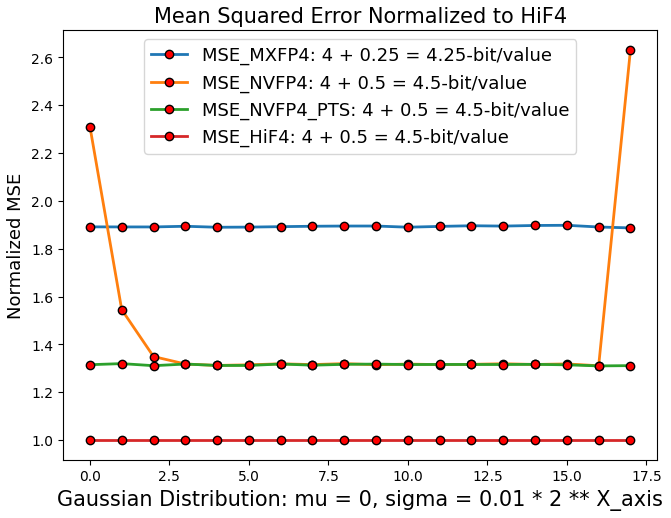
\includegraphics[width=\linewidth]{Fig/MSE-BFP4.png}
  \caption{Quantization Error Comparison of 4-bit BFP Formats}
  \label{MSE-BFP4}
\end{figure}

\subsection{Quantization Error Evaluation}
We generated 18 high-precision Gaussian-distributed random 
matrices of size $1024 \times 1024$, 
each with zero mean and standard deviation $\sigma = 0.01 
\times 2^x$, where $x \in [0, 17]$. 
Every matrix was converted to three 4-bit BFP formats. 
HiF4 followed Algorithm \ref{BF16 to HiF4}. 
MXFP4 adopted the method described in \cite{Rouhani2023}. 
NVFP4 employed E4M3 scaling to normalize the peak magnitude 
of each group to 6, the representable upper bound of E2M1. 
Since only NVFP4 lacks sufficient dynamic range and requires 
additional software-based PTS, 
two versions were prepared for fair comparison: 
a direct cast and a pipeline that first scales each tensor's 
peak magnitude to 2688 and then quantizes to NVFP4 \cite{Alvarez2025}. 
We computed the mean squared error (MSE) relative to the 
original high-precision matrix for each format 
and normalized the results with respect to HiF4. 

Figure \ref{MSE-BFP4} depicts the quantization error 
of HiF4, MXFP4, and NVFP4. 
When data values approach the numeric bounds of NVFP4, 
overflow and underflow cause the quantization error to 
increase significantly. 
Applying PTS before format conversion can eliminate this 
precision loss. 
In contrast, HiF4 and MXFP4 do not require PTS, thus  
incurring no additional quantization overhead. 
Excluding NVFP4's fluctuation, the MSE ratio across the 
three 4-bit BFP formats remains stable: 
\[
\text{HiF4 : NVFP4 : MXFP4} = 1 : 1.32 : 1.89 
\]
Note that although the Gaussian distribution matches the 
centralized nature of the data in neural networks, 
the quantization error may vary in practical scenarios. 
The experimental results serve as a quantitative reference 
for analyzing the accuracy of different 4-bit BFP formats. 

\subsection{Dot Product Evaluation}

\begin{figure*}[htbp]
  \centering
  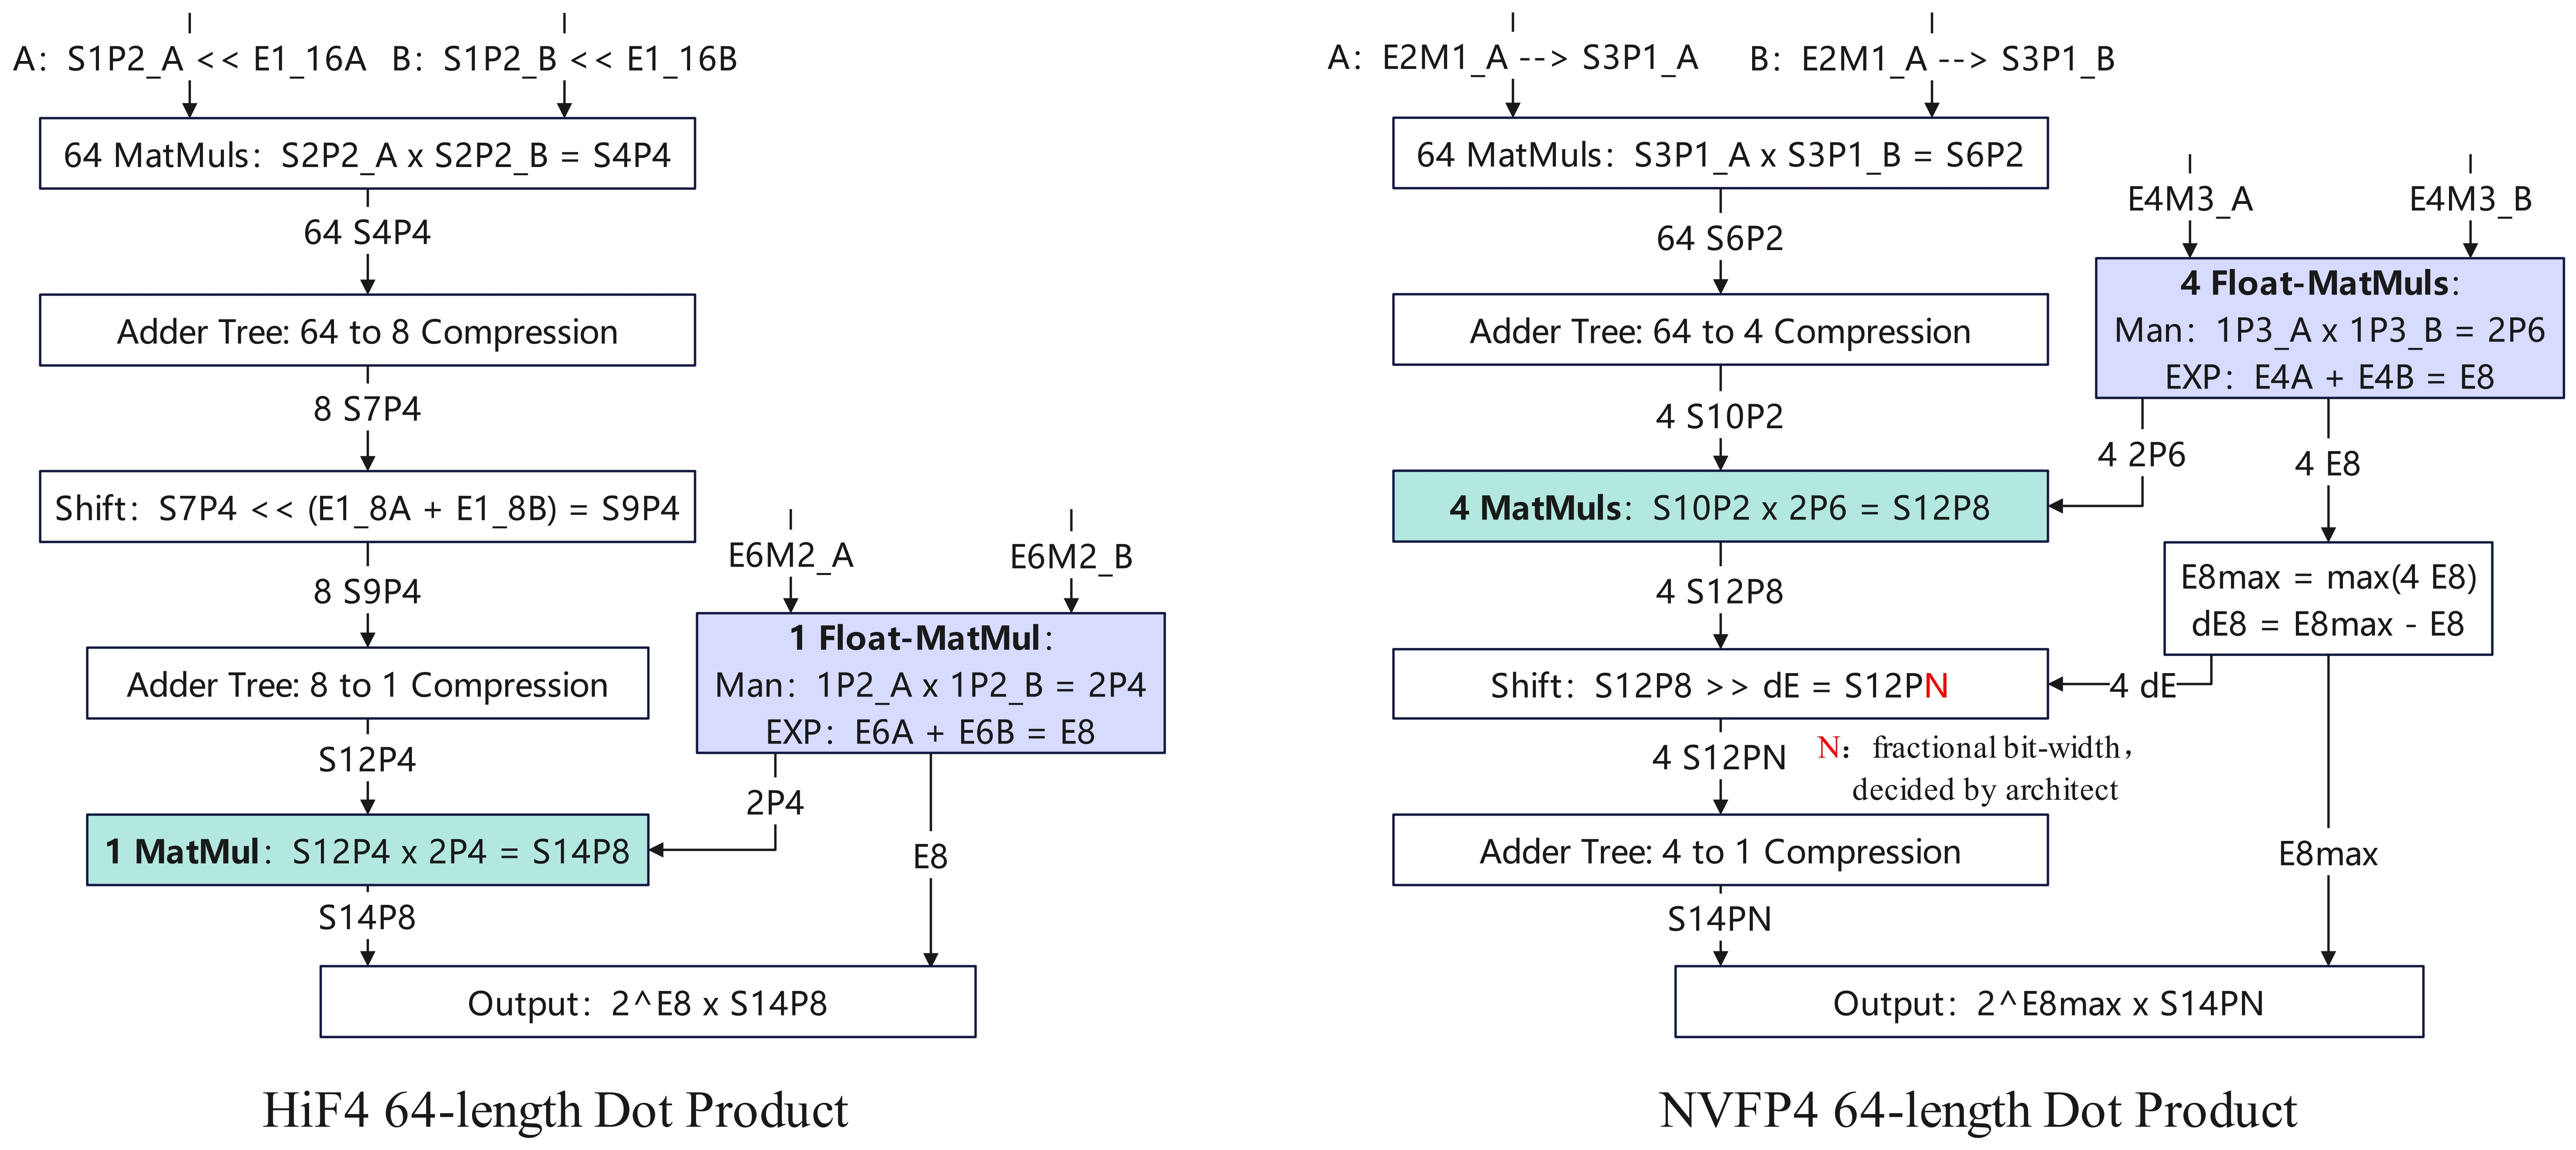
\includegraphics[width=17cm]{Fig/BFP4-MatMul.jpg}
  \caption{Compute Flow of 64-length Dot Product for HiF4 and NVFP4}
  \label{BFP4-MatMul}
\end{figure*}

Let A: 
$\{E6M2^{(A)}, E1\_8^{(A)}, E1\_16^{(A)}, S1P2\_64^{(A)}\}$ 
and B: $\{E6M2^{(B)}, E1\_8^{(B)}, E1\_16^{(B)}, S1P2\_64^{(B)}\}$ 
denote the two HiF4 units. 
The dot product of A and B should be computed as follows: 
\begin{align}
  Dot(A, B)& = E6M2^{(A)} \times E6M2^{(B)} \times \notag \\
  &\sum_{i=1}^8  2^{(E1\_8^{(A)}[i] + E1\_8^{(B)}[i])} \times \notag \\
  &\sum_{j = 2i-1}^{2i} 2^{(E1\_16^{(A)}[j] + E1\_16^{(B)}[j])} \times \notag \\
  &\sum_{k = 4j-3}^{4j} (S1P2\_64^{(A)}[k] \times S1P2\_64^{(B)}[k])
  \label{Dot-Product}
\end{align}
% To support general dot product and general matrix multiplication, 
% a FP32 accumulator is further needed:
% \begin{equation}
%   C_{FP32} = C_{FP32} + Dot(A, B)
%   \label{Accumulator}
% \end{equation}
In hardware, a processing element (PE) that performs a K-length 
dot product and accumulation in parallel is a fundamental building 
block of matrix-compute units, 
such as Nvidia GPU's Tensor Cores \cite{Nvidia2017} and 
Ascend NPU's Cube Cores \cite{Liao2019}.
To double the computing power of 4-bit BFP formats relative to 
8-bit floating-point formats, 
both Tensor Cores and Cube Cores now require PEs to support 
64-length dot products \cite{Nvidia2025, Eric2025}.
Under these conditions, a single pair of HiF4 units suffices to 
match the PE input width, 
since their group size is exactly 64. 
In contrast, four pairs of NVFP4 units are required to support 
a 64-length dot product in a PE, 
because their group size is only 16.
Next, we briefly analyze the compute flow of HiF4 and NVFP4 in 
a 64-length dot product to reveal their differences in power and 
area consumption.

For the HiF4 dot product, level-2 and level-3 micro-exponents 
can be implemented as simple left-shift operations in hardware. 
There are many opportunities to absorb the micro-exponents into 
the computations related to the S1P2 elements, 
depending on the implementation strategy. 
In our example compute flow, we directly absorb the level-3 
micro-exponents into the S1P2 elements prior to multiplications. 
In this way, multiplier inputs become 5-bit integers, 
which can be denoted as S2P2 (for simplicity, we continue using 
the SXPY notation). 
Similarly, E2M1 elements in NVFP4 are converted into 
5-bit integers (S3P1) before multiplications. 
Figure \ref{BFP4-MatMul} illustrates the compute flow of 
64-length dot product for both formats. 
During the compression from 64 products to a single S12P4 output, 
HiF4 employs pure integer arithmetic, 
requiring only one small floating-point multiplier and one large 
integer multiplier at the final stage of the accumulation tree. 
In contrast, NVFP4 retains integer operations only during the 
reduction from 64 products to four S10P2 outputs, after which four  
small floating-point multipliers and four large integer multipliers 
are required. 
The final accumulation from four partial results to the output is 
then performed entirely in floating-point. 
Consequently, HiF4 eliminates six multipliers and simplifies the 
accumulation process compared with NVFP4. 

In practice, 4-bit BFP formats are integrated into 
existing dot-product units originally optimized for 16-bit 
(FP16 and BF16) and 8-bit (INT8 and Float8) formats. 
Although resource sharing is feasible across different precision 
modes, high-precision formats do not require intermediate and final 
multipliers within the accumulation tree. 
Thus, the additional multipliers introduced by floating-point 
metadata E6M2 and E4M3 incur extra hardware overhead. 
As a result, for 64-length dot product, HiF4 occupies only 
approximately one-third the incremental area of NVFP4 and reduces 
the power consumption by about 10\%. 
In summary, HiF4 enables a more area- and power-efficient 
implementation for matrix multiplication. 
